% multiple1902 <multiple1902@gmail.com>
% intro.tex
% Copyright 2011~2012, multiple1902 (Weisi Dai)
% https://code.google.com/p/xjtuthesis/
% 
% It is strongly recommended that you read documentations located at
%   http://code.google.com/p/xjtuthesis/wiki/Landing?tm=6
% in advance of your compilation if you have not read them before.
%
% This work may be distributed and/or modified under the
% conditions of the LaTeX Project Public License, either version 1.3
% of this license or (at your option) any later version.
% The latest version of this license is in
%   http://www.latex-project.org/lppl.txt
% and version 1.3 or later is part of all distributions of LaTeX
% version 2005/12/01 or later.
%
% This work has the LPPL maintenance status `maintained'.
% 
% The Current Maintainer of this work is Weisi Dai.
%

\chapter{系统实现及测试}
\echapter{Implementation}
\label{ImplementationChapter}
\section{客户端函数库实现及测试}
\par
在描述了客户端函数库应当实现的功能和其类图结构之后,这里给出客户端函数库基于C\#语言的实现情况的概述。
语法上,Java和C\#是十分相似的。甚至有别的项目提供了Java到C\#语言的翻译工具\footnote{可用的工具之一的链接,http://sourceforge.net/projects/j2cstranslator/}。然而经过测试,翻译器的结果是不理想的。因此,作者基于Java函数库的语义,完成了C\#客户端函数库的实现。实现过程中需要注意的是两种语言提供的低层支持不同,例如Java.NIO中提供了可以用作缓存基础数据结构的高效字节缓存ByteBuffer类的实现;Java提供的传输层TCP网络接口与C\#提供的接口略有不同;Java应用RSA公钥算法加解密,附加、核实签名的方式不同于C\#;以及Java的异常抛出、处理机制和C\#不相同 。
\par
为了依然保持对上层的统一接口,作者及同事按照Java语言的文档在C\#语言中分别实现了上述不同之处。对应在源代码文件中,ByteBuffer的实现在ByteBuffer.cs中的net.named-data.jndn.ByteBuffer类;传输层接口的实现在TcpTransport.cs中的net.named-data.jndn.transport.TcpTransport类;Java的RSA私钥功能的辅助类的实现在net.named-data.jndn.security.certificate.PrivateKey类;异常处理机制体现在每个函数的抛出错误部分的重写。
\par
函数库部分其它的实现与Java源码的逻辑近似。但是个别函数,例如获取当前的操作系统时间等采用了特定语言的调用。
客户端函数库附带了几个测试文件,用以测试函数库是否工作正常。TestEchoConsumer.cs实现Echo请求名称对应的数据应答;TestEncodeDecodeData测试用选择的编码格式编码、解码数据应答;TestEncodeDecodeForwardingEntry测试用选择的编码格式编码、解码数据请求的选择符;TestEncodeDecodeInterest测试用选择的编码格式编码、解码数据请求;TestGetAsync测试向指定的接口发送数据请求,是否可以得到预料的数据应答;TestPublishAsyncNdnx测试向本地的NDN daemon注册数据Echo请求前缀,并根据收到的Echo数据请求做以相应的数据应答。
\par
目前C\#客户端函数库的实现情况,除了从DER格式字节读入公钥、私钥外,已与5月31日的Java客户端函数库\footnote{对应的Github Commit链接,https://github.com/named-data/jndn/commit/3d59135aa1c1398a524b0d37c5fafdf26e149349}保持一致。 目前由于NDN daemon并不为各个应用发布它们应该使用的证书,而只要求可以利用数据应答的发布者提供的公钥能够核实数据应答的签名即可,所以C\#客户端函数库采用了一组提前预设的公钥私钥对,而不是从给定的DER格式字节读入。
\par
关于C\#客户端函数库的实现另外值得一提的一点是,作者原本尝试了利用IKVM工具\footnote{IKVM工具的链接,http://www.ikvm.net/},将Java源码编译对象指定为DotNet Assembly;或是利用IronPython\footnote{http://ironpython.net/}将Python源码编译对象指定为DotNet Assembly,但是两个方案都行不通。前者的问题在于编译成的DotNet Assembly需要基于IKVM提供的DotNet Assembly,而后者包含Unity3D引擎不支持的DotNet基础库。后者的问题在于Unity3D支持的C\#语言版本过低,如果不利用C\# 4.0提供的dynamic关键字,IronPython编译结果会使得基本的函数调用代码很不工整。
\par
本部分的实现和简单说明可以在作者的Github站点\footnote{ndn-dot-net开发者函数库的作者Github链接,https://github.com/zhehaowang/ndn-dot-net}上找到。
\section{同步模块实现及测试}
\par
完成了同步模块功能的流程描述和类图描述后,本部分讲述同步模块的开发实现。同步模块实现采用的项目命名空间是remap.NDNMOG.DiscoveryModule,并包含子命名空间remap.NDNMOG.DiscoveryModule.Test。命名空间的命名满足C\#函数库命名空间命名的一般要求。设计部分描述的类均属于前一个命名空间。
\par
由于设计部分的功能描述已较为明确,实现时需要关注的重点有哈希函数、编码方式的选择,参数的选择,和对上层提供的接口。
\subsection{哈希函数、编码方式和参数选择}
\setcounter{subsubsection}{0}
\par
由于本文涉及的名称字符串数量不多,长度较少,本文首先对所有字符串做以异或,得到一个字符串后采用FNV哈希计算Digest值。哈希函数的实现继承自只包含功能的父类,因此哈希函数可以较为轻松的修改。
\par
在选择完哈希函数后,需要对得到的整型做以向URI的转换。本文采用了Base64的编码方式,将整型二进制直接编码为字符串。Base64不足的部分采取补0。在优化中提到的\ref{MultiLevelOptimizationSection}部分后,编码的格式如下。
\newline
\centerline{<type - relative octant index - digest - relative octant index 2 - digest 2>}
\par
本应用涉及到的主要参数有。
\subsubsection{32位FNV哈希常量}
大质数值设置为16777619;偏移量值为2166136261;
\subsubsection{超时时间和间隔时间常量}
发现请求的超时时间为10秒,发现请求的最小间隔为3秒,应答的新鲜时间为20秒;位置请求的超时时间为0.5秒,位置请求的最小间隔为0.25秒,应答的新鲜时间为1秒;
\subsubsection{八叉树层数及可以注册请求前缀的有效层数}
八叉树对虚拟环境的默认划分层数为7层,从第5层开始可以注册前缀;
\subsubsection{掉线判定的超时位置请求个数}
连续收到20个位置请求超时将认为节点掉线。
\par
经测试,以上参数的选取在网络广播流量上和更新速度上,即从实时性和大规模可拓展性的要求上而言是比较合适的。
\par
最后描述一点实现过程中为了降低和游戏应用的耦合度所做的优化。由于同步模块是独立的DotNet Assembly(mono dll),其应该被游戏应用调用。游戏应用应向其提供本地对象的位置,并读出同步模块提供的周围其它对象的位置及行动,从而进行渲染。为了减少二者间的耦合度,同步模块的用例类可以接收调用者传入的一个回调函数。因此,在游戏应用中实例化用例类时,将渲染入口传入,即可以利用同步模块的工作结果进行周围其它对象的渲染。
\par
本部分的实现和简单说明可以在作者的Github站点\footnote{同步模块的作者Github链接,https://github.com/zhehaowang/DiscoveryModule}上找到。
\subsection{测试}
\label{TestResults}
\par
同步模块的测试分为2个部分。模块本身包含了测试文件,用以模拟产生一个用例类,并进行发现,同时输出八叉树的情况和Base64编码的哈希值,以观察模块基本功能是否工作正常。模块还在多台机器运行的实际的游戏应用中进行了测试。实际测试的环境如下。
为多个运行Mac OSX 10.8和10.7的计算机,分别生成游戏二进制文件,通过配置文件为生成的二进制文件赋予用于发布位置、行动等信息的用例名。在两台计算机上配置并运行ndnd-tlv。本部分将给出应用运行的步骤和界面,测试的结果和理论分析将在\ref{EvaluationChapter}部分给出。
\par
这里由于篇幅的限制,作者不讨论ndnx或是ndnd-tlv的安装、配置过程;其与ndn-cpp函数库,ndn-cxx函数库的关系;以及其与ccnd、ndnd和NFD的兼容性问题。该过程中可能遇到的问题在项目对应的redmine站点\footnote{安装配置ndnd-tlv的相关信息链接,redmine.named-data.net/projects/ndnd-tlv/wiki},或是作者的github代码工程的readme中可以找到。
\par
之后为二者都添加到一个NDN公用节点aleph.ndn.ucla.edu的TCP连接。这里应当注意要使用该节点提供的可创建路由回路的前缀列表中的前缀,从而使得多个节点互相发送的发现数据请求可以被该节点正常前递到应该收到请求的节点。添加连接的命令类似ndndc add /ndn/edu/ucla/remap tcp aleph.ndn.ucla.edu,其中/ndn/edu/ucla/remap是aleph提前配置好可以供本应用注册的名称前缀。
\par
图\ref{fig:ApplicationConfiguration}为游戏应用开始前的配置界面。
\begin{figure}[h!]
	\centering
	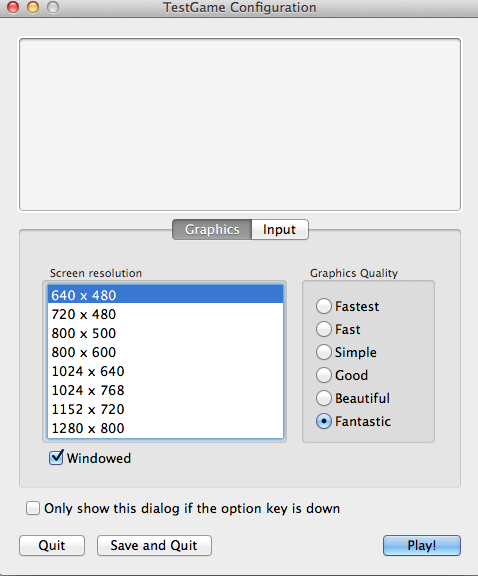
\includegraphics[width=6.67cm]{GameConfiguration}
	\caption{游戏应用配置界面图}
	\label{fig:ApplicationConfiguration}
\end{figure}
\par
完成了游戏应用相关常数的配置后,图\ref{fig:ApplicationRunning}为游戏应用的运行界面。界面体现了测试用的简单游戏环境。正中央的葫芦状物体是第三人称视角下的本节点所主持的游戏实体,即运行该应用的玩家在游戏虚拟世界中的化身(Player Avatar)。由于该应用刚开始运行,发现过程尚未完成。
\begin{figure}[h!]
	\centering
	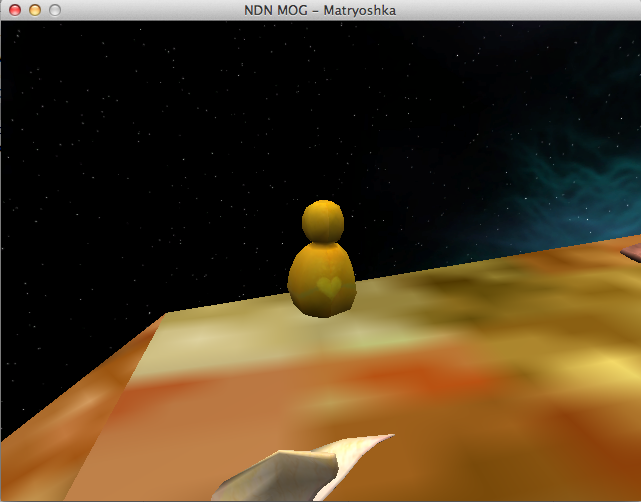
\includegraphics[width=6.67cm]{GameInstance}
	\caption{游戏应用开始运行时界面图}
	\label{fig:ApplicationRunning}
\end{figure}
\par
图\ref{fig:ApplicationDiscovering}是在上图反映的游戏实体进行了运动,并且通过命名数据网络的请求、应答交互,即本文重点描述的方案的步骤后,发现周围存在的其它节点主持的游戏实体的应用界面图。图中出现的另一个葫芦状物体为通过发现过程发现的另一物体。图中出现的其它物体为游戏中的非玩家角色,这些角色的数据应当动态的由特定的节点存储。为了简单起见,当前的视线中这些节点的数据全部在运行游戏的第一个节点进行存储。
\begin{figure}[h!]
	\centering
	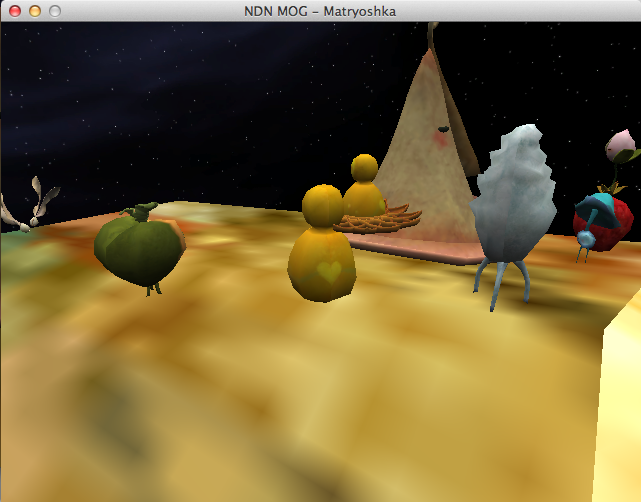
\includegraphics[width=6.67cm]{GameDiscovery}
	\caption{游戏应用开始运行时界面图}
	\label{fig:ApplicationDiscovering}
\end{figure}
\par
上述应用为设计方案提供了实际测试的环境。测试结果的数据汇总和分析将在\ref{EvaluationChapter}部分给出。测试所用的单元测试文件包含在对应的功能模块的Github库中;游戏测试文件可以在作者的Github库\footnote{游戏应用的Github链接,https://github.com/zhehaowang/NDNMOG-live}中找到。
\par
在完成了实现过程的叙述后,本文对设计方案做出了测试结果的实际分析、理论分析,以及诸多优化。
\section{本章小结}
本章提供了本应用涵盖的三层,即开发者函数库层,同步模块层和游戏应用层的实现细节和初步的测试结果,并对测试结果做以了详细的分析。实现细节并没有具体到每个类实现的功能和实现时作出的选择。细节性的内容可以在每层对应的Github链接中看到代码和说明。